\documentclass[apectratio=43,unicode]{beamer}
\usetheme{Moscow}

\usepackage[utf8]{inputenc}
\usepackage[T2A]{fontenc}
\usepackage[main=russian,english]{babel}

\usepackage{amsmath,amssymb}

\renewcommand{\thefootnote}{\fnsymbol{footnote}}
\hypersetup{pdfauthor={Ivan Tsybulin}}

\usepackage{euler}
\usepackage{mathtools}

\graphicspath{{images//},{source//}}

\title[Задача Коши]{Задача Коши для обыкновенного дифференциального уравнения}
\author[Цыбулин И.В.]{Скалько Юрий Иванович\\
\textbf{Цыбулин Иван}}
\date{}

\newcommand{\colorhref}[2]{\href{#1}{\textcolor{miptbase!30!black}{#2}}}

\begin{document}

\begin{frame}[plain]
\titlepage
\end{frame}

\def\L{\mathcal{L}}

\section{Обыкновенные дифференциальные уравнения}
\subsection{Задача Коши}
\begin{frame}\frametitle{Задача Коши для ОДУ}
	Дано обыкновенное дифференциальное уравнение 1го порядка и начальное условие
	\begin{align*}
	\frac{dy(t)}{dt} &= G(t, y(t))\\
	y(0) &= y_0
	\end{align*}
	Требуется найти решение $y(t)$ при $t \in [0, T]$
\end{frame}

\begin{frame}\frametitle{Приближение непрерывной функции}
	Решением задачи коши является некоторая непрерывная функция $y(t)$.

	Поскольку вычислительная техника не может работать с произвольными непрерывными функциями,
	требуется упростить вид функции решения $y(t)$.
\end{frame}

\subsection{Разностная задача}
\begin{frame}\frametitle{Сетка}
	Введем на отрезке $[0, T]$, на котором решается задача Коши, сетку из точек $t_n$.
	\begin{itemize}
	\item Если $\tau = t_{n+1} - t_n$ одинаков для всех $n$, то сетка называется 
		равномерной. При этом шаг сетки $\tau$ является постоянным.
	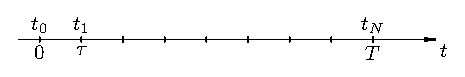
\includegraphics[width=.8\textwidth]{grid-0.eps}
	\item Иначе, сетка называется неравномерной
	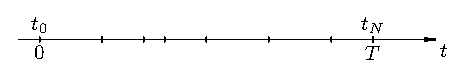
\includegraphics[width=.8\textwidth]{grid-1.eps}
	\end{itemize}
\end{frame}

\begin{frame}\frametitle{Сеточная функция}
	Сеточная функция, в отличие от непрерывной, является элементом конечномерного пространства $\mathbb{R}^n$

	Операция получения из непрерывной функции $y(t)$ сеточной функции $\mathbf{u}$ 
	называется \emph{проецированием} и обозначается квадратными скобками.
	$$
	u_n = y(t_n) = [y]_n
	$$
	\begin{figure}%
	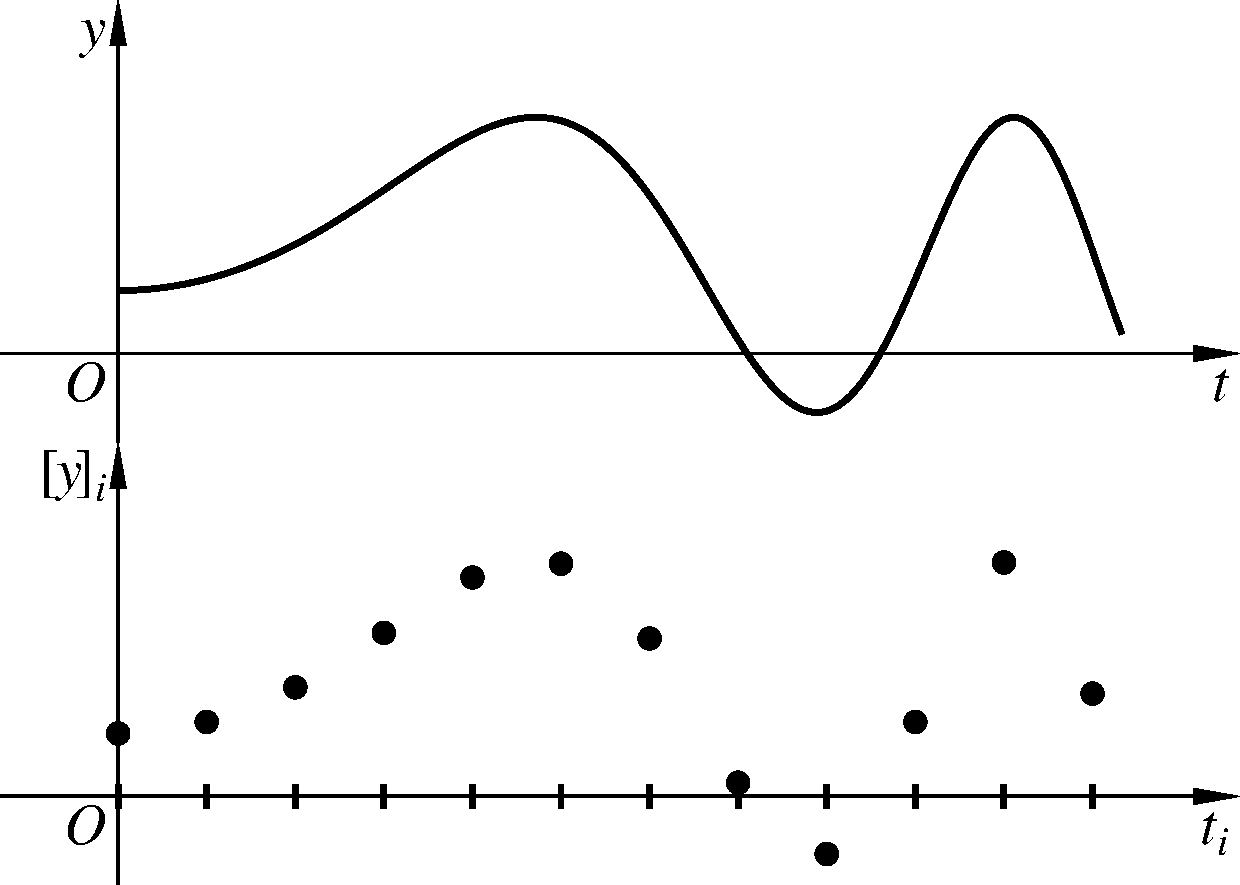
\includegraphics[height=0.5\textheight]{proj.pdf}%
	\end{figure}
\end{frame}

\begin{frame}\frametitle{Операторная форма записи}
	Задачу Коши
	\begin{align*}
	\frac{dy(t)}{dt} &= G(t, y(t))\\
	y(0) &= y_0
	\end{align*}
	можно записать в операторном виде
	$$
	\L y(t) = f(t)
	$$
	Оператор $\L$ состоит из дифференциального оператора и начального условия
	$$
	\L y(t) = \left\{
	\begin{array}{l}
		\displaystyle \frac{dy(t)}{dt} - G(t, y(t))\\
		\\
		y(0)
	\end{array}
	\right.
	\quad,\quad
	f(t) = \left\{
	\begin{array}{l}
		0\\
		\\
		y_0
	\end{array}
	\right.	
	$$
\end{frame}

\def\Lh{{\L^{(\tau)}}}
\begin{frame}\frametitle{Разностная задача}
	Поскольку неизвестной функцией является теперь \emph{сеточная функция} $[y]$ необходимо переформулировать исходную задачу 
	Коши для непрерывной функции, в некоторую, похожую, \emph{разностную} задачу.
	\pause

	По аналогии с общим видом задачи Коши
	$$
	\L y(t) = f(t)
	$$
	рассмотрим разностную задачу
	$$
	\Lh \mathbf{u} = \mathbf{g}
	$$
	Здесь $\mathbf{u}$ и $\mathbf{g}$ --- сеточные функции, а $\Lh$ --- разностный оператор
\end{frame}

\frametitle{Сравнение различных задач}
\begin{frame}
	Допустим имеется дифференциальная задача Коши
	$$
	\L y(t) = f(t)
	$$
	и разностная задача
	$$
	\Lh \mathbf{u} = \mathbf{g}
	$$
	\begin{itemize}
	\item Как убедиться, что эти задачи действительно <<похожи>>, и главное, что
<<похожи>> \emph{решения} этих задач?
	\pause

	\item Как вообще можно сравнить между собой непрерывную функцию $y(t)$ и сеточную функцию $\mathbf{u}$?
	\end{itemize}
\end{frame}

\subsection{Аппроксимация и сходимость}
\begin{frame}\frametitle{Сравнение решений}
	Сравнивать решения разных задач из разных пространств напрямую невозможно.

	Вместо этого необходимо перевести решения в некоторое другое пространство и сравнивать уже элементы
	одного и того же пространства.
	\pause

	Оказывается, удобно сравнивать решения именно в пространстве сеточных функций. Для этого необходимо перевести
	непрерывное решение $y(t)$ в пространство сеточных функций. Операция проектирования как раз и служит для этого
	$$
	y(t) \rightarrow [y]
	$$
\end{frame}

\begin{frame}\frametitle{Сходимость}
	Можно легко сравнить проекцию решения дифференциальной задачи $[y]_n$ и решение разностной задачи $u_n$. 
	$$
	\varepsilon = \|[y] - \mathbf{u}\| = \max_n |[y]_n - u_n|
	$$

	При изменении шага сетки $\tau$ будут получаться различные разностные задачи 
	с различными решениями $\mathbf{u}^{(\tau)}$. 
	$$
	\varepsilon^{(\tau)} = \|[y] - \mathbf{u}^{(\tau)}\| = \max_n |[y]_n - u_n^{(\tau)}|
	$$
	
	Если $\varepsilon^{(\tau)} \rightarrow 0$ при $\tau \rightarrow 0$, то говорят о \emph{сходимости} решений 
	разностной задачи к решению дифференциальной задачи. Если при этом $\varepsilon^{(\tau)} = O(\tau^k)$, 
	то говорят о сходимости $k$-го порядка
\end{frame}

\begin{frame}\frametitle{Пример}
	Рассмотрим задачу Коши
	$$
		y' = y, \quad y(0) = 1, \quad t \in [0, T]
	$$
	и разностную задачу
	$$
		u_{n+1} = (1 + \tau) u_n, \quad u_0 = 1, \quad n = \overline{0,N}, \quad \tau = \frac{T}{N}
	$$
	Решения обеих задач легко находятся: $y(t) = e^t$ и $u_n = \left(1+\tau\right)^n$
	$$
	\varepsilon^{(\tau)} = e^T - \left(1 + \tau\right)^N = e^T - e^{N \ln \left(1+\tau\right)} = 
	$$
	$$
	= e^T - e^{T - \frac{T\tau}{2} + o\left(\tau\right)} = e^T \left(1 - e^{1-\frac{\tau}{2}+o(\tau)} \right) = 
	\frac{e^T}{2}\tau + o(\tau) = O(\tau)
	$$
	Решение разностной задачи сходится к решению дифференциальной задачи с первым порядком
\end{frame}

\begin{frame}\frametitle{Сходимость}
	Наличие сходимости позволяет находить решение дифференциальной задачи с любой точностью, взяв 
	в качестве решения решение разностной задачи. 
	
	Например, в примере для вычисления $y(1)$ можно было взять $u_N$ при достаточно большом $N$.
	\pause
	
	Однако, напрямую проверять сходимость бессмысленно, так как требуется иметь решение исходной 
	дифференциальной задачи.
	
	Рассмотрим другие свойства, которые можно проверить не обладая точным решением
\end{frame}

\begin{frame}\frametitle{Аппроксимация}
	Аппроксимация показывает насколько хорошо решение дифференциальной задачи 
	$$
	\L y(t) = f(t)
	$$
	удовлетворяет разностной задаче
	$$
	\Lh \mathbf{u} = \mathbf{g}
	$$
	\pause
	Поскольку решение дифференциальной задачи является непрерывной функцией, а разностная задача 
	сформулирована в терминах сеточной функции, необходимо вначале спроецировать решение $y(t)$ на сетку,
	а уже после этого подставлять в разностную задачу $\Lh \mathbf{u} = \mathbf{g}$
	\pause
	
	Поскольку, в общем случае, такая функция не обязана быть решением разностной задачи, в правой части появится невязка
	$$
	\Lh [y] = \mathbf{g} + \delta \mathbf{g}
	$$
\end{frame}

\begin{frame}\frametitle{Ошибка аппроксимации}
	$$
	\Lh [y] = \mathbf{g} + \delta \mathbf{g}
	$$
	
	Величина невязки в правой части называется ошибкой аппроксимации
	$$
	\delta g = \|\delta \mathbf{g}\|
	$$
	
	Если эта величина стремится к нулю при $\tau \rightarrow 0$, то говорят что разностная задача \emph{аппроксимирует}
	дифференциальную, а если дополнительно $\delta g = O(\tau^k)$, то говорят, что имеет место аппроксимация $k$-го порядка
	\pause
	
	Но исходя из определения не ясно, как найти ошибку аппроксимации не обладая 
	точным решением $y(t)$ или его проекцией $[y]$
\end{frame}

\subsection{Исследование аппроксимации}
\begin{frame}\frametitle{Нахождение ошибки аппроксимации}
	Выберем произвольную точку $t^*$. Удачный выбор точки позволит впоследствии сильно сократить объем вычислений.
	
	Разностный оператор $\Lh$ действуя на сеточную функцию $[y]$, на самом деле, действует на значения $y(t_n)$.
	Каждое из этих значений можно представить по формуле Тейлора в виде
	$$
	y(t_n) = y(t^*) + (t_n-t^*) y'(t^*) + \frac{(t_n-t^*)^2}{2} y''(t^*) + \dots + \frac{(t_n-t^*)^k}{k!} y^{(k)}(\xi_n)
	$$
	
	Отметим, что все производные функции $y(t)$ взяты в одной и той же точке $t^*$. 
	Вспомним, что $y(t)$ является на самом деле	решением задачи Коши, поэтому 
	\begin{align*}
	y'(t^*) &= G(t^*, y(t^*))\\
	y''(t^*) &= G_t(t^*, y(t^*))+G_y(t^*, y(t^*))G(t^*, y(t^*))\\
	&\vdots
	\end{align*}
\end{frame}

\begin{frame}\frametitle{Нахождение ошибки аппроксимации}
	Итак, имея представление в виде формулы Тейлора
	$$
	y(t_n) = y(t^*) + (t_n-t^*) y'(t^*) + \frac{(t_n-t^*)^2}{2} y''(t^*) + \dots + \frac{(t_n-t^*)^k}{k!} y^{(k)}(\xi_n)
	$$
	а также связи
	\begin{align*}
	y'(t^*) &= G(t^*, y(t^*))\\
	y''(t^*) &= G'_t(t^*, y(t^*))+G'_y(t^*, y(t^*))G(t^*, y(t^*))\\
	&\vdots
	\end{align*}
	можно выразить ошибку аппроксимации $\delta g_n$ как 
	$$
	\delta g_n = F_0(y(t^*)) + \tau F_1(y(t^*)) + \dots + \frac{\tau^{k-1}}{{k-1}!} F_{k-1}(y(t^*)) + O(\tau^{k})
	$$
	Если все функции $F_0(y), F_1(y), ..., F_k(y)$ тождественно равны нулю, то ошибка аппроксимации будет иметь порядок $O(\tau^k)$
\end{frame}

\begin{frame}\frametitle{Пример}
	Рассмотрим задачу Коши
	$$
	y' = t \sin y, \quad y(0) = 1, \quad t \in [0, T]
	$$
	и разностную задачу
	$$
	\frac{u_{n+1} - u_n}{\tau} = \tau\left(n+\frac{1}{2}\right)\sin\left(u_n + \frac{\tau^2 n}{2} 
		\sin u_n\right), \quad u_0 = 1
	$$
	Подставим $\mathbf{u} = [y]$
	\begin{align*}
	&\frac{[y]_{n+1} - [y]_n}{\tau} = \tau\left(n+\frac{1}{2}\right)\sin\left([y]_n + \frac{\tau^2 n}{2} 
		\sin [y]_n\right) + \delta g_{n+1}\\
	&[y]_0 = 1 + \delta g_0
	\end{align*}
	
	Заметим, что начальное условие является частью разностного оператора и тоже может иметь невязку!
\end{frame}

\begin{frame}\frametitle{Пример}
	Задача Коши
	$$
	y' = t \sin y, \quad y(0) = 1, \quad t \in [0, T]
	$$
	Разностная задача
	\begin{align*}
	&\frac{[y]_{n+1} - [y]_n}{\tau} = \tau\left(n+\frac{1}{2}\right)\sin\left([y]_n + \frac{\tau^2 n}{2} 
		\sin [y]_n\right) + \delta g_{n+1}\\
	&[y]_0 = 1 + \delta g_0
	\end{align*}
	Представим $[y]_{n+1}$ в виде формулы Тейлора в окрестности точки $t_n$
	$$
	[y]_{n+1} = [y]_n + \tau [y']_n + \frac{\tau^2}{2} [y'']_n + O(\tau^3)
	$$
	$$
	\frac{[y]_{n+1} - [y]_n}{\tau} = [y']_n + \frac{\tau}{2} [y'']_n + O(\tau^2)
	$$
\end{frame}

\begin{frame}\frametitle{Пример}
	Задача Коши
	$$
	y' = t \sin y, \quad y(0) = 1, \quad t \in [0, T]
	$$
	Разностная задача
	\begin{align*}
	&\frac{[y]_{n+1} - [y]_n}{\tau} = \tau\left(n+\frac{1}{2}\right)\sin\left([y]_n + \frac{\tau^2 n}{2} 
		\sin [y]_n\right) + \delta g_{n+1}\\
	&[y]_0 = 1 + \delta g_0
	\end{align*}
	Воспользуемся дифференциальным уравнением
	\begin{align*}
	[y']_n &= n \tau \sin [y]_n = O(1)\qquad (n = O(\tau^{-1}))\\
	[y'']_n &= \sin [y]_n + (n\tau)^2 \cos [y]_n \sin[y]_n = O(1)
	\end{align*}
	$$
	\frac{[y]_{n+1} - [y]_n}{\tau} = [y']_n + \frac{\tau}{2} [y'']_n + O(\tau^2) =
	$$
	$$
	= n\tau \sin [y]_n  + \frac{\tau}{2}\left(\sin [y]_n + (n\tau)^2 \cos [y]_n \sin[y]_n\right) + O(\tau^2)
	$$
\end{frame}

\begin{frame}\frametitle{Пример}
	Задача Коши
	$$
	y' = t \sin y, \quad y(0) = 1, \quad t \in [0, T]
	$$
	Разностная задача
	\begin{align*}
	&\frac{[y]_{n+1} - [y]_n}{\tau} = \tau\left(n+\frac{1}{2}\right)\sin\left([y]_n + \frac{\tau^2 n}{2}
		\sin [y]_n\right) + \delta g_{n+1}\\
	&[y]_0 = 1 + \delta g_0
	\end{align*}
	Представим правую часть в виде формулы Тейлора
	$$
	\tau\left(n+\frac{1}{2}\right)\sin\left([y]_n + \frac{\tau^2 n}{2} \sin [y]_n\right) = 
	$$
	$$
	= (n\tau)\sin [y]_n + \frac{\tau}{2}\sin [y]_n + \frac{\tau}{2}(n\tau)^2\cos[y]_n\sin[y]_n + O(\tau^2)
	$$
\end{frame}

\begin{frame}\frametitle{Пример}
	Задача Коши
	$$
	y' = t \sin y, \quad y(0) = 1, \quad t \in [0, T]
	$$
	Разностная задача
	\begin{align*}
	&\frac{[y]_{n+1} - [y]_n}{\tau} = \tau\left(n+\frac{1}{2}\right)\sin\left([y]_n + \frac{\tau^2 n}{2} 
		\sin [y]_n\right) + \delta g_{n+1}\\
	&[y]_0 = 1 + \delta g_0
	\end{align*}
	Сравнивая разложения для правой и левой частей, получаем
	\begin{align*}
	\delta g_0 &= 0\\
	\delta g_{n+1} &= O(\tau^2)
	\end{align*}
	$$
	\delta g = \|\delta \mathbf{g}\| = O(\tau^2)
	$$
	Разностная задача аппроксимирует дифференциальную со вторым порядком
\end{frame}

\begin{frame}\frametitle{Аппроксимация начальных условий}
	Не стоит забывать проверять аппроксимацию начальных условий. Хотя в предыдущем примере 
	аппроксимация с любым порядком начального условия была очевидна, так бывает не всегда.
	
	Например, изменив в разностной задаче начальное условие с 
	$$
	u_0 = 1
	$$
	на
	$$
	u_0 = 1+2\tau
	$$
	мы бы все равно получили аппроксимирующую задачу, но порядок аппроксимации был бы уже первый, так как
	\begin{align*}
	\delta g_0 &= 2\tau = O(\tau)\\
	\delta g_{n+1} &= O(\tau^2)
	\end{align*}
	$$
	\delta g = \|\delta g_n\| = O(\tau)
	$$
\end{frame}

\subsection{Устойчивость}
\begin{frame}\frametitle{Устойчивость}
	При проверке аппроксимации мы убеждаемся, что решение $[y]$ <<почти>> удовлетворяет задаче
	$$
	\Lh \mathbf{u} = \mathbf{g}
	$$
	Рассмотрим возмущенную задачу
	$$
	\Lh \mathbf{u} = \mathbf{g} + \delta \mathbf{g}
	$$
	Эти задачи отличаются только небольшим возмущением правой части. Если это возмущение не сильно повлияет
	на решение, можно утверждать, что $\mathbf{u} \approx \mathbf{v}$. Если допустить единственность 
	решения возмущенной задачи, то
	$$
	\Lh \mathbf{v} = \mathbf{g} + \delta \mathbf{g} = \Lh [y]
	$$
	и $[y] = \mathbf{v}$, а следовательно и $\mathbf{u} \approx [y]$.
\end{frame}

\begin{frame}\frametitle{Устойчивость}
	Введем понятие \emph{устойчивой} разностной задачи. Задача 
	$$
	\Lh \mathbf{u} = \mathbf{g}
	$$
	называется устойчивой, если для для небольших возмущений $\delta g_n$ задача
	$$
	\Lh \mathbf{u} = \mathbf{g} + \delta \mathbf{g}
	$$
	имеет единственное решение $v_n$, причем
	$$
	\|\mathbf{v} - \mathbf{u}\| < C \|\delta \mathbf{g}\|
	$$
	а константа $C$ не зависит от $\tau$
\end{frame}

\begin{frame}\frametitle{Теорема Рябенького-Филиппова-Лакса}
	\begin{block}{Основная теорема вычислительной математики}
		Пусть устойчивая с коэффициентом $C$ разностная задача 
		$$
		\Lh \mathbf{u} = \mathbf{g}
		$$
		аппроксимирует задачу
		$$
		\L y(t) = f(t)
		$$
		с ошибкой аппроксимации $\|\delta \mathbf{g}\| = \delta g < D \tau^k$. Тогда решения разностной задачи 
		сходятся к решению дифференциальной, причем для ошибки сходимости справедлива оценка
		$$
		\varepsilon^{(\tau)} < C D \tau^k \mathop{\longrightarrow}_{\tau \rightarrow 0} 0
		$$
	\end{block}
\end{frame}

\begin{frame}\frametitle{Исследование устойчивости}
	В отличие от нахождения ошибки аппроксимации, единого способа проверки устойчивости нет.

	Докажем устойчивость разностной задачи
	$$
	\frac{u_{n+1}-u_n}{\tau} = G\left(t_n+\frac{\tau}{2},u_n + \frac{\tau}{2}G(t_n, u_n)\right),\quad u_0 = y_0
	$$
	в предположении, что по второму аргументу функция $G$ Липшицева, то есть
	$$
	|G(t, u) - G(t, v)| < L|u-v|
	$$
	Введем функцию
	$$
	F(t, u, \tau) = u+\tau G\left(t+\frac{\tau}{2},u+\frac{\tau}{2}G(t,u)\right)
	$$
\end{frame}

\begin{frame}\frametitle{Исследование устойчивости}
	$$
	F(t, u, \tau) = u+\tau G\left(t+\frac{\tau}{2},u+\frac{\tau}{2}G(t,u)\right)
	$$
	Функция $F(t,u,\tau)$ также Липшицева по $u$
	$$
	|F(t,u,\tau)-F(t,v,\tau)| < |u-v| \left(1 + L\tau\left(1+\frac{L\tau}{2}\right)\right) < e^{L\tau} |u-v|
	$$
	Разностную задачу можно переписать в виде
	$$
	u_{n+1} = F(t_n, u_n, \tau), \quad u_0 = y_0
	$$
	При возмущении исходной задачи на $\delta \mathbf{g}$ получается задача
	$$
	v_{n+1} = F(t_n, v_n, \tau) + \tau \delta g_{n+1}, \quad v_0 = y_0 + \delta g_0
	$$
	Отметим множитель $\tau$ перед $\delta g_{n+1}$. Он появился при умножении исходной задачи на $\tau$
\end{frame}

\begin{frame}\frametitle{Исследование устойчивости}
	$$
	|F(t,u,\tau)-F(t,v,\tau)| < e^{L\tau} |u-v|
	$$
	\begin{align*}
	u_{n+1} &= F(t_n, u_n, \tau), \quad u_0 = y_0\\
	v_{n+1} &= F(t_n, v_n, \tau) + \tau \delta g_{n+1}, \quad v_0 = y_0 + \delta g_0
	\end{align*}
	Справедлива следующая цепочка оценок
	\begin{align*}
	|u_0 - v_0| &= |\delta g_0|\\
	|u_1 - v_1| &= |F(t_0, u_0, \tau)-F(t_0, v_0, \tau) - \tau \delta g_1| < 
		e^{L\tau} |\delta g_0| + \tau |\delta g_1|\\
	|u_2 - v_2| &= |F(t_1, u_1, \tau)-F(t_1, v_1, \tau) - \tau \delta g_2| < 
		e^{2L\tau} |\delta g_0| + \\
				& \hspace{.63\textwidth} e^{L\tau} \tau |\delta g_1| + \tau |\delta g_2|\\
	|u_n - v_n| &< e^{n L\tau}|\delta g_0| + \frac{e^{n L\tau}-1}{e^{L\tau}-1}\tau\max_{n>0} |\delta g_n|
	\end{align*}
	$$\|u_n - v_n\| \lesssim e^{LT} |\delta g_0| + \frac{e^{LT}-1}{L} \max_{n>0} |\delta g_n| \leq
	\max\left(e^{LT}, \frac{e^{LT}-1}{L}\right) \|\delta g\|$$
\end{frame}

\begin{frame}\frametitle{Исследование устойчивости}
	Для данной задачи единственность решения очевидна (все неизвестные $u_n$ вычисляются последовательно), 
	а константой устойчивости будет
	$$
	\max\left(e^{CT}, \frac{e^{CT}-1}{C}\right)
	$$

	Заметим, что от $\tau$ она не зависит. По определению, данная задача устойчива.
\end{frame}

\begin{frame}[plain]
  \begin{center}
  {\Huge Спасибо за внимание!}
  \vspace{8ex}

  Цыбулин Иван

  e-mail: \colorhref{mailto:tsybulin@crec.mipt.ru}{tsybulin@crec.mipt.ru}
  \end{center}
\end{frame}
\end{document}
